\documentclass[journal,a4paper]{IEEEtran}
\usepackage{graphicx}
\usepackage{xcolor}
\usepackage{xeCJK}
%\usepackage{CJK}
\usepackage{fontspec}
\usepackage{geometry}
\usepackage{fancyhdr}
\usepackage{mdframed}
\usepackage{listings}
\usepackage{amsmath,amssymb,mathrsfs}
\usepackage{multirow}
\usepackage{float}
\usepackage{booktabs}
\usepackage{url}
\usepackage{hyperref}
\usepackage{array}
\usepackage{enumerate}
\usepackage{subfig}
\usepackage{longtable}

\bibliographystyle{IEEEtran}
\newtheorem{myDef}{\textbf{Definition}}
\newtheorem{myPro}{\textbf{Problem}}

\linespread{1.3}

\geometry{left=2.5cm,right=2.5cm,top=2.5cm,bottom=2.5cm}

\title{\huge{若干马氏链蒙特卡洛采样方法的比较与分析}}

\author{王禹~~无48~~2014011241}

\begin{document}

	\maketitle
	\begin{abstract}

		本文对估计受限玻尔兹曼机(RBM)的归一化常数经常使用的四种马氏蒙特卡洛抽样方法进行了复现改进,一定程度上提高了抽样方法的效率,并对这四种抽样方法的稳定性进行了比较分析。我使用MNIST手写数字数据库对四种方法进行了测试与比较,以此来对四种抽样方法的效率与性能进行评估与分析。

	\end{abstract}


	\section{Introduction}
	 手写体数字识别一直是一个研究热门问题,因为其应用广泛,且对识别的误识别率有着较高的要求。传统的分析方法是通过提取手写数字像素获得高维数特征集,再利用类似PCA等特征选择方法,筛选出维度较低的特征,在利用这些较低维度的特征训练神经网络,从而获得分类器。而本文所进行比较的四种方法,则均是直接将$ 28 \times 28 = 784$个像素点作为特征,输入到受限玻尔兹曼机(RBM)的观测变量端,并将该一层网络训练为分类器,训练过程中需要计算RBM的归一化常数。由于观测变量有784个,隐变量可以取任意数目,故最少共有$ 2^784 $种观测变量与隐变量的组合情况。这个数字对于计算机系统而言是巨大的,因此使用遍历方法计算归一化常数会有巨大的代价,所以需要使用合适的抽样方法对归一化常数进行逼近与估计。

	 本文所比较的四种采样方法分为三种。以AIS(Annealed Importance Sampling)\cite{salakhutdinov2009learning}为代表的方法采用的是构造了一个易于计算归一化常数的RBM,然后构造一系列过渡温度因子,通过温度过渡,逐渐计算出目标RBM的归一化常数。以RTS(Rao-Blackwellized Tempered Sampling)\cite{carlson2016partition}和SAMS(Self-adjusted mixture sampling)\cite{tan2015optimally}为代表的方法,同样是构造了一个易于计算归一化常数的RBM,也同样构造出了一系列温度过渡因子。不同的是,其通过迭代将所有温度过渡过程的归一化常数同时计算。经过足够多的次数和,归一化常数趋于稳定,去除归一化常数数列的最后一项,即为目标RBM的归一化常数。	而TAP(Thouless-Anderson-Palmer)\cite{gabrie2015training}所采用的是则是将归一化常数的ln值,即自由能,泰勒展开。因为无论是玻尔兹曼机还是受限玻尔兹曼机(RBM),都应当是系统能量最低的状态,即稳定状态。因此使用迭代法获得稳定v,h的能量状态后,将其带入总RBM自由能的泰勒展开式,进行一定的近似截取,即可获得总的自由能,即归一化常数的值。
	\section{Model}
	本实验的基本模型为受限玻尔兹曼机(RBM),是深度学习的重要基础模型之一,其结构如图Fig.~\ref{fig1}所示:

		\begin{figure}[h]
		\centering
		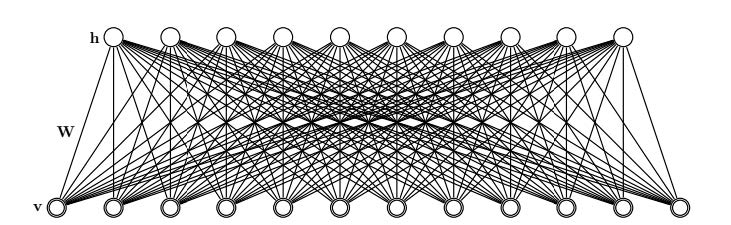
\includegraphics[width=0.5\textwidth]{1.jpg}
		\caption{RBM结构模型}
		\label{fig1}
		\end{figure}
	RBM由一层观测变量和一层隐变量构成,变量均为0,1取值。模型的能量符合物理中的玻尔兹曼分布,即:
		\begin{align}
		 & E(v,h;\theta) \notag \\
		 & =  -v^TWh-b^Tv-a^Th \notag \\
		 & =  -	\sum_{i}{\sum_j{ W_{ij}v_ih_j - \sum_i b_iv_i - \sum_j a_jh_j}}
		\end{align}
	而RBM模型观测变量和隐变量的联合分布为:
		\begin{align}
		p(v,h;\theta) = \frac{1}{Z(\theta)}e^{-E(v,h;\theta)}
		\end{align}
	其中,
		\begin{align}
		Z(\theta) = \sum_{v} \sum_h e^{-E(v,h;\theta)}
		\end{align}
	为归一化常数。

	\section{Methods}
	\subsection{Basic Method - MCMC}

	在简述计算RBM归一化常数的采样方法之前,将先行简述一般的MCMC(Markov Chain Monte Carlo)方法。
	\begin{myDef}
		为要模拟服从给定分布T的随机变量,用生成一个易于实现的不可约遍历链$ X=\{X_n,n\geq O\} $作为随机样本,使其平稳分布为$ \pi $的方法,称为马氏链蒙特卡罗方法.
	\end{myDef}
	而Metropolis-Hastings算法则为MCMC方法的一个改进,具体表述如下:

	\begin{table}[h]
		\begin{tabular}{ll}
			\hline
			\multicolumn{2}{l}{\textbf{Algorithm 1:}Metropolis-Hastings Algorithm} \\
			\hline
			1: & 设$\pi = (\pi(i), i\in S)$为任意给定的概率分布,\\
			 & 而$ T = (T(i,j), i,j\in S)$为任选的易于实现 \\
			 & 的条概率转移矩阵\\
			2: & 给定$\pi = (X_n\in S, n\geq 0)$,由$T(X_n,·) $ \\
			 & 抽取Y,并计算\\
			 & $ \rho = min\{ 1,\pi(Y)T(Y,X_n)/(\pi(x)T(X_n,Y) \} $ \\
			3: & 抽取$ U \sim U[0,1]$,若$ U <\rho$, \\
			 & 则$ X_{n+1} = Y$,否则舍去Y,返回步骤2。\\
			\hline
		\end{tabular}
		\caption{Metropolis-Hastings Algorithm}
		\label{tab1}
	\end{table}

	使用上述方法可以获得所需分布的抽样样本。

	\subsection{RBM归一化参数与最似然概率估计}

	在讲述具体的抽样方法之前,需要首先说明一下抽样方法。四种归一化参数的估计方法中,除了TAP外,都采用了类似的转移采样方法,具体模型如图Fig.~\ref{fig2}所示:
	\begin{figure}[h]
		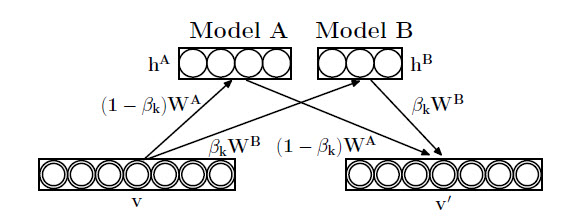
\includegraphics[width = 0.5\textwidth]{2.jpg}
		\caption{Transition Operation Model}
		\label{fig2}
	\end{figure}
	即构造一组$[0,1]$的温度过渡值,从易于计算归一化常数的温度模型,过渡到目标模型。而在中间的某一个温度过渡过程下,由上述模型可以算出转移得到的下一个观测变量$v'$的值。而对应到具体的数学表达式为:
	\begin{flalign}
	p(h_j^A=1|\mathbf{v}) & = g\left((1-\beta_k)\left(\sum_i W_{ij}^A v_i +a_j^A\right)\right) \\
	\label{equ3}
%	\end{flalign}
%	\begin{equation}
	p(h_j^B=1|\mathbf{v}) & = g\left(\beta_k\left(\sum_i W_{ij}^B v_i +a_j^B\right)\right) \\
	\label{equ4}
	%\end{equation}
%	\begin{flalign}
	p(v_i'=1|\mathbf{h}) & = g((1-\beta_k)(\sum_i W_{ij}^A v_i + a_j^A) \\
	 & +\beta_k(\sum_i W_{ij}^B v_i +a_j^B))
    \label{equ5}
	\end{flalign}
	其中,$g(x)=\frac{1}{1+e^{-x}}$,为 logistic function。

	\subsubsection{AIS\cite{salakhutdinov2009learning}}
		AIS 方法使用一系列过渡的$\beta_k$值,将易于计算归一化常数的RBM过渡到目标RBM。本文实现的具体算法如Table~\ref{tab2}所示:
		\begin{table}[h]
			\begin{tabular}{ll}
				\hline
				\multicolumn{2}{l}{\textbf{Algorithm 2:}Annealed Importance Sampling} \\
				\hline
				1: & 从$ 0=\beta_0<\beta_1<...<\beta_K=1$中随机选择一个$\beta_k$\\
				2: & 用选择的$\beta_k$采样一个$x_1$,满足最初的易于计算的\\
				 & RBM的$P_A$ \\
				3: & for $k = 1 : K-1$ do \\
				4: & ~~~~通过$T_k$转移矩阵,以及目前的$x_k$,采样$x_{k+1}$。\\
				5: & end \\
				6: & 令$ \omega_k = \frac{Z_{k+1}}{Z_k} = \frac{P_{k+1}^*(x)}{P_{k+1}^*(x)}$,其中$ x \sim P_k$\\
				7: & $ \prod_{k=1}^K\omega_k = \frac{Z_B}{Z_A}$,便可以获得最终结果\\

				\hline
			\end{tabular}
			\caption{AIS Algorithm}
			\label{tab2}
		\end{table}

		原始的算法中,$ \omega_k $ 一项表示成:$ \omega_k = \frac{Z_{k+1}}{Z_k} =\frac{1}{M} \sum_{i = 1}^{M} \frac{P_{k+1}^*(x^{(i)})}{P_{k+1}^*(x^{(i)})}$,$x^{(i)} \sim P_k$。即原始算法对每一种$beta_k$值均作了M次抽样,之后将M次的结果作了平均。但是本算法中,将M取为1,也得到了较好的结果。
		而$P_k^*(\mathbf{v})$ 可以用如下的等式计算:
		\begin{align}
		 & P_k^*(\mathbf{v}) = e^{\beta_k\sum_i b_i^Bv_i} \left[\prod_{j=1}^{F_B} \left(1+e^{\beta_k(\sum_i W_{ij}^Bv_i+a_j^B)}\right)\right] \notag\\
		 & \times e^{(1-\beta_k)\sum_i b_i^Av_i} \left[\prod_{j=1}^{F_A} \left(1+e^{(1-\beta_k)(\sum_i W_{ij}^Av_i+a_j^A)}\right)\right]
		 \label{equ8}
		\end{align}

		具体的实验,实验结果以及分析见下一节。

	\subsubsection{TAP\cite{gabrie2015training}}
		由前述可知,RBM的联合分布为$P(v,h)=Z^{-1}e^{-E(v,h)}$,$Z$为归一化常数。取对数后,可得
		\begin{equation}
			\mathcal{L} = lnP(v) = - F^c(v)+F
		\end{equation}
		其中,$F = -lnZ$为RBM的自由能,$F^c(v)= -n(\sum_he^{-E(v,h)})$为RBM的钳制自由能。本文关心重点为归一化常数的估计,因此,我们所关心的是RBM的\textbf{自由能}。而吉布斯-波尔兹曼分布的\textbf{能量}在基于配置s的情况下$E(s) = -\sum_ia_is_i-\sum_{(i,j)}W_{ij}s_is_j$。
		为了降低计算\textbf{自由能}的计算量。首先恢复玻尔兹曼分布中的温度$\beta$对于基于玻尔兹曼分布的模型的影响,因为大多数模型中,将温度设定为常数1,从而忽略温度的影响。之后,将\textbf{能量}用外部辅助场$q$重写,可以得到$-\beta F[q] = ln \sum_se^{-\beta E(s)+ \beta\sum_iq_is_i} $ 而在经过Legendre变换,引入共轭变量$ m  = {m_i}$后,可以获得
		\begin{equation}
		 -\beta \Gamma[m]= -\beta \max_q[F[q]+\sum_iq_im_i]
		\end{equation}
		而\textbf{自由能}则为应该是经过Legendre变换后$q=0$的状态在经过反Legendre变换可得,即
		\begin{equation}
		 -\beta F= -\beta F[q=0] = -\beta \min_m[ \Gamma[m]] = -\beta  \Gamma[m^*]
		\end{equation}
		而对于任意的$A(\beta,m) \equiv -\beta\Gamma[m] $,展开后可得:
		\begin{align}
		A(\beta,m) & = A(0,m) + \beta \frac{\partial A(\beta,m)}{\partial\beta}\big|_{\beta=0} \notag \\
		& + \frac{\beta^2}{2}\frac{\partial^2A(\beta,m)}{\partial\beta^2}\big|_{\beta=0} + ...
		\end{align}
		因此可以得到:
		\begin{align}
		-\beta\Gamma(m)= &-\sum_i[m_i\ln m_i + (1-m_i)\ln(1-m_i)] \notag \\
		& +\beta \sum_i a_im_i + \beta \sum_{(i,j)} W_{ij}m_im_j \notag \\
		& +\frac{\beta^2}{2} \sum_{(i,j)} W_{ij}^2(m_i-m_i^2)(m_j -m_j^2) \notag \\
		& +\frac{2\beta^2}{3} \sum_{(i,j)} W_{ij}^3(m_i-m_i^2)(\frac{1}{2}-m_i) \notag \\
		& (m_j -m_j^2)(\frac{1}{2}-m_j) + ...
		\end{align}

		而回到RBM模型,其\textbf{能量}的Legendre变换应该有如下的形式:
		\begin{align}
		\Gamma(m^v,m^h) \eqsim & -S(m^v,m^h) -\sum_i a_im_i^v  -\sum_i b_jm_j^h \notag \\
		& -\sum_{i,j} W_{ij}m_i^vm_j^h \notag \\
		& -\sum_{i,j} \frac{W_{ij}^2}{2}(m_i^v-(m_i^v)^2)(m_j^h -(m_j^h)^2) \notag \\
		& -\sum_{i,j} \frac{2}{3}  W_{ij}^3(m_i-m_i^2)(\frac{1}{2}-m_i) \notag \\
		& (m_j -m_j^2)(\frac{1}{2}-m_j) - ...
		\label{equ1}
		\end{align}
		这里将温度$\beta$设置为1,且精确到了三阶近似,若是只需要二阶近似,则把最后一项略去即可。
		而为了得到\textbf{自由能},需要式(\ref{equ1})能够取的最小值。因此需要$\frac{d\Gamma}{dm}=0$。因此可以通过如下的迭代式得到带入计算的$m^v,m^h$:
		\begin{flalign}
			m_j^h[t+1] & \leftarrow g[b_j+\sum_i W_{ij}m_i^v[t] \notag \\
			& - \sum_i W_{ij}^2\left(m_j^h[t]-\frac{1}{2}\right)(m_i^v[t]-m_i^v[t]^2) \notag \\
			& + \sum_i W_{ij}^3(m_i^v[t]-m_i^v[t]^2)(\frac{1}{2} - m_i^v[t]) \notag\\
			& (2(m_j^h[t]^2-m_j^h[t])+\frac{1}{3})] \\
			m_i^v[t+1] & \leftarrow g[a_i+\sum_j W_{ij}m_j^h[t+1] \notag \\
			& - \sum_j W_{ij}^2\left(m_i^v[t]-\frac{1}{2}\right)(m_j^h[t+1]-(m_j^h[t+1])^2)  \notag \\
			& + \sum_j W_{ij}^3(m_j^h[t+1]-m_j^h[t+1]^2)(\frac{1}{2}-m_j^h[t+1]) \notag\\
			& (2(m_i^v[t]^2-m_i^v[t])+\frac{1}{3})]
		\end{flalign}
	\subsubsection{RTS\cite{carlson2016partition} and SAMS\cite{tan2015optimally}}
	RTS方法与SAMS方法比较类似,在此一并介绍。
	首先先介绍RTS方法。该方法也是构造出一系列温度过渡因子$ 0=\beta_1<\beta_2<...<\beta_K=1$如同AIS所示。在该温度的情况下的中间分布情况与上述的AIS一致,即
	\begin{equation}
		p(x|\beta_k)=\frac{f_k(x)}{Z_k}
	\end{equation}
	式中的$f_k(x)=P_A^*(x)^{1-\beta_k}P_B^*(x)^{\beta_k}$,其中$P_A^*,P_B^*$即为式(\ref{equ8})中所示。
	式中的$Z_k$为温度处在$\beta_k$的情况下的归一化常数。
	RTS算法的核心便是通过多次迭代,同时更新所有温度过渡因子下的归一化常数。每次迭代的过程中,会同时对温度过渡因子$\beta$和观测变量$v$进行抽样。本算法中对观测变量的采样方法与本节开头的方法相同,即式(\ref{equ3}),(\ref{equ4}),(\ref{equ5})。这里主要叙述$\beta$的抽样方法。

	当$\beta \in \beta_k$是一个随机变量时,假定有一个先验概率$r(\beta_k)=r_k$,那么$x,\beta_k$的联合分布则如下表示:
	\begin{align}
	p(x,\beta_k) & = p(x|\beta_k)r_k, \\
	& = \frac{f_k(x)r_k}{Z_k}
	\end{align}
	由于$Z_k$是我们需要求的,并不知道,因此我们可以定义$\hat{Z_k}$则
	\begin{equation}
	q(x,\beta_k) \propto \frac{f_k(x)r_k}{\hat{Z_k}}
	\end{equation}
	由于联合分布已经知道,文献\cite{carlson2016partition}定义出:
	\begin{equation}
	q(\beta_k|x) = \frac{f_k(x)r_k/\hat{Z_k}}{\sum_{l=1}^{K} f_l(x)r_l/\hat{Z_l}}
	\end{equation}
	有了上述的概率分布,我们便可以通过采样出的$x_k$,对下一次迭代使用的$\beta_s$进行抽样。即$q(\beta_1),q(\beta_2),...,q(\beta_K)$依次按照其值,在$[0,1]$的轴上占据一定位置。取一符合$U(0,1)$的随机变量,该变量落入哪一个$q(\beta_k)$的区间,则将该$\beta_k$作为下一次迭代使用的$\beta$。而每次迭代中,则采用$ \hat{Z_k^{RTS}} = \hat{Z_k}\frac{r_1}{r_k}\frac{\hat{c_k}}{\hat{c_1}}$,其中$\hat{c_k}=\frac{1}{N} \sum_{i=1}^N q(\beta_k|x^{(i)})$。

	但是原始文章所采用的$q(\beta_k|x;\hat{Z_k})$收敛效果并不好,因此我将$q(\beta_k|x;\hat{Z_k})$定义时进行了改进。由文献\cite{salakhutdinov2009learning}中指出,对于任意一个$beta_k$,其未归一化的中间概率分布应当为式(\ref{equ8})所示。将其归一化之后,应当与$q(\beta_k|x;\hat{Z_k})$等价。而将$q(\beta_k|x;\hat{Z_k})$中的易于计算归一化常数的RBM的影响项从$q(\beta_k|x;\hat{Z_k})$中去除,即将$q(\beta_k|x;\hat{Z_k})$除以$Z_A^{1-\beta_k}$。经过这样的处理后,收敛效果得到了较好的提升。

	具体的算法步骤见下表TABLE~\ref{tab3}:
	\begin{table}[h]
		\begin{tabular}{ll}
			\hline
			\multicolumn{2}{l}{\textbf{Algorithm 3:}Rao-Blackwellized Tempered Sampling} \\
			\hline
			1: & 初始化$ 0=\beta_0<\beta_1<...<\beta_K=1$\\
			   & 初始化$\ln Z_k=0,k=2,...,K$ \\
			   & 初始化$\hat{c_k}=0,k=2,...,K$ \\
			2:& while $max{abs(\hat{c_k}-\frac{1}{K})}>Tlimit$\\
			3: & ~~~~for $i = 1 : N$ do \\
			4: & ~~~~~~~~通过转移矩阵(即式(\ref{equ3})(\ref{equ4})(\ref{equ5})),以及目前 \\
			   & ~~~~~~~~的$\beta_k$,采样$x$。\\
			5: & ~~~~~~~~通过$q(\beta_k|x;\hat{Z_k})$采样下一次迭代的$\beta$ \\
			6: & ~~~~~~~~更新$\hat{c_k} \leftarrow \hat{c_k} + \frac{1}{N} q(\beta_k|x)$ \\
			7: & ~~~~end for\\
			8: & ~~~~更新$\hat{Z_k}^{RTS} \leftarrow \hat{Z_k}\frac{r_1}{r_k} \frac{\hat{c_k}}{\hat{c_1}}$ \\
			9: & end while\\

			\hline
		\end{tabular}
		\caption{RTS Algorithm}
		\label{tab3}
	\end{table}

	而SAMS与RTS大体相似,算法步骤也基本相似,但是具体来说,根据文献\cite{tan2015optimally}所示,其更新$Z_k$的方法以及抽样$\beta$的方法不一样。这里先指出$\beta$的抽样方法不同之处。如上所示,RTS的$\beta$抽样方法,是全局抽样(global jump),即下一次抽样的$\beta_k$的位置可以是那组$\beta$的任意值,但是根据文献\cite{salakhutdinov2009learning}所示,SAMS的抽样方法是局部抽样(local jump),即每次抽取的下次的$\beta$值只能是本次$\beta$的相邻的$\beta$值。但是根据测试,这种local jump的抽样方法收敛速度较慢,需要牺牲效率,以更多地迭代次数才能得到准确的结果。因此我将此方法改进,仍然采用global jump的方式,进行$\beta$抽样。
	而SAMS的归一化常数更新的方法与RTS也不相同。RTS通过两层循环,更新$\hat{c}$后,再新$\hat{Z}$的方法。而SAMS的更新方法则如下描述:
	令$\zeta = \ln Z$,则:
	\begin{align}
		& \zeta^{(t-\frac{1}{2})} = \zeta^{(t-1)} + \notag \\ 
		& \lambda\{\frac{q_1(·;\hat{Z^{(t-1)}})}{r_1},\frac{q_2(·;\hat{Z^{(t-1)}})}{r_2},...,\frac{q_K(·;\hat{Z^{(t-1)}})}{r_K}\},
	\end{align}
	\begin{equation}
		\zeta^{(t)} = \zeta^{(t-\frac{1}{2})} - \zeta_1^{(t-\frac{1}{2})} \notag
	\end{equation}
	其中$\zeta_1^{(t-\frac{1}{2})}$为$\zeta^{(t-\frac{1}{2})}$的第一项,而$\lambda$满足如下的关系,以增加收敛的速度:
	
	$\lambda = \Big\{ \begin{matrix}
			\min(\pi_j,t^{-\beta}) & if~t \leq t_0 \\
			\min\{\pi_j,(t-t_0+t_0^{\beta})^{-1}\} & if~t > t_0 \\
			\end{matrix} $
	
	而此处的$q_k$也仍采用了我在RTS中叙述的改进,将RBM A的能量部分除去,以获得更好的收敛效果。
	
	\section{Analysis of Method \& Results}
	由于程序的运行时间和机器的配置有着较大的关系,本文的仿真实验,都是在CPU为i7-6700@3.4GHz,内存16GB的电脑上运行的。
	\subsection{MCMC}
	为了验证MCMC,我们对二维高斯的相关系数的进行估计。

	\begin{myPro}
		用 Metropolis-Hastings算法,对下述二维高斯分布进行随机采样
		\begin{equation*}
		\mathscr{N}\left\{\begin{pmatrix}x_1\\x_2\end{pmatrix}\bigg|\begin{pmatrix} 5 \\ 10 \end{pmatrix},\begin{pmatrix} 1 & 1\\1 & 4\end{pmatrix}\right\}
		\end{equation*}
		使用生成的随机样本来估计二维高斯函数的相关系数,并与真值比较。
	\end{myPro}

		由于这里抽样的数字为一个二维向量,且在$\mathbb{R}^2$上式连续。因此T取有限大小会对转移产生误差。因此在本题中,没有构造出真实的转移矩阵T,而是假定转移矩阵T为一个所有元素都相同且符合马尔科夫转移性质的矩阵,即每一行相加为1。这种情况下,上述算法Table~\ref{tab1}中的$ T(Y,X_n) $与$T(X_n,Y)$相消,故只需要计算即将抽样的样本点的概率密度与前一个已经确认的样本点的概率密度作比值,在与一个在$ [0,1] $均匀分布的随机变量作比较后,来判断是否转移成功即可。而由于T为完全均匀的转移矩阵,因此下一个抽样点的抽取应当完全随机抽取。这里为了提高抽取的命中率,我将$x_1$与$x_2$分别按照独立的两个一维高斯分布抽取随机数,一维高斯分布的均值与标准差均来自于二维随机分布中的均值与协方差矩阵。同样,这样的抽样方法,也使得最终的结果的相关系数与抽样点的个数无关,不会随着抽样点的数目增加而变得更加接近真值。
		
		理论的相关系数应当为0.5。使用MATLAB仿真相关系数分布在$[0.484,0.497]$之间。
		为评判MCMC的准确性,多次试验,每次实验均抽取5万个计算所得结果的方差,结果如下:
		\begin{center}
		\begin{tabular}{c|c}
			\hline
			运行次数 & 结果方差\\
			\hline
			5 & $5.49\times10^{-6}$ \\
			10 & $2.20\times10^{-5}$ \\
			20 & $3.69\times10^{-5}$ \\
			50 & $1.74\times10^{-5}$ \\
			100 & $1.67\times10^{-5}$ \\
			\hline
		\end{tabular}
		\end{center}
		首先分析本方法的准确性,由上述结果可见,多次运行本MCMC方法的方差非常小,为$10^{-5}$量级,而相关系数为$10^{-1}$量级。因此可以认为该MCMC抽样方法准确性相当高,几乎没有误差,同时,其抽样出的结果与相关系数与真值也非常接近。
		其次是对算法效率的分析。运行一次生成5万个抽样点的MATLAB程序需要大概1s到2s的时间,主要时间开销在抽样主程序上。其次为了实现该算法,完成了一个计算二维正太分布概率密度的函数,该函数调用较为高效,3s的时间可以调用300万次。总体程序的效率较高。
	\subsection{AIS}
		在本实验实现AIS方法时,划分的温度过渡因子越细致,即$\beta$的集越大,所得到的结果越加精细,估计值更加贴近真值,但相对的运算的代价会变大,计算速度会变慢。具体的算法,在前述部分已经得到了讲解,在此对算法进行分析。
		
		首先分析程序效率。为了提高程序效率,令$ \omega_k = \frac{Z_{k+1}}{Z_k} =\frac{1}{M} \sum_{i = 1}^{M} \frac{P_{k+1}^*(x^{(i)})}{P_{k+1}^*(x^{(i)})}$中的$M=1$,既可以减少抽样次数,提高程序效率,也可以获得较好的结果。在尽可能获得准确的结果的情况下,令$\beta$的取值更加精细。根据实验结果来看,$\beta$的精细程度需要根据RBM的隐变量数目来动态决定。根据实验结果,对于10个隐变量取$\beta$数组的元素数为10万,20个隐变量取为50万,100个隐变量取为50万,500个隐变量取为60万。而根据MATLAB本身的运算特性,尽可能的将所有的循环改写成为矩阵运算后,程序的运行效率得到了大大的提高。经过MATLAB仿真测试,h10的模型,运行时间为10s;h20的模型运行时间为60s;h100的模型运行时间为100s;h500的模型运行时间为。而该函数主要耗费效率的部分是抽样算法,抽出下一个观测变量的运算,以及一些求和运算,这些运算都无法避免或者使用矩阵乘法提高运算效率。
		
		再分析程序的准确性,将AIS函数循环20次,计算归一化常数的方差值,所得的结果如下表TABLE~和下图Fig.所示:
		\begin{tabular}{cc}
			Model & Var \\
			h10 & 0.1939 \\
			h20 & 19.4639 \\
			h100 & 0.1089 \\
			h500 & \\
		\end{tabular}
		通过上述结果可以看出,AIS的结果相对而言是非常稳定的,每次产生的归一化常数的值也较为相似。可以看出,AIS算法除了花费的时间非常长之外,获得结果的准确性非常高。

	\subsection{TAP}
		而对TAP算法进行分析时,可以发现由于TAP算法是一种近似算法,其估计的归一化常数值与真值之间的误差几乎不变,多次运行试验时得到的一组估计归一化常数的方差也非常小。而且方差随着近似程度的增加,会逐渐变小。
		
		本文随附代码实现了TAP的二阶近似算法TAP2与三阶近似算法TAP3。两个算法的运行性能结果如下表所示:
		\begin{tabular}{cccc}
			Model & TAP2 Var & TAP3 Var & Consuming Time \\
			h10 & 0.2188 & & \\
			h20 & 0.2188 & & \\
			h100 & 0.2188 & & \\
			h500 & 0.2188 & & \\
		\end{tabular}


	\subsection{RTS}
		RTS的结果收敛性较差,波动性也较高。这个和RTS算法中的易于计算归一化常数的RBM参数设置有关。最开始,作者尝试使用全为0的参数设置为RBM A的参数。然而,这种情况下RTS算法并不收敛,其估算出的误差呈现周期性的波动。因此,我尝试改变RBM A的一个或两个参数。由文献\cite{salakhutdinov2009learning}中指出,当$W_A$取为全0矩阵时,有$P^A(\mathbf{v})=\prod_ip_A(v_i)=\prod\frac{1}{1+e^{-b_i}}$。由此可以解出$b_i = \ln \frac{P_i^A}{1-P_i^A}$。因此,在此将$b^A$设定为如下的值。令$b^A=\ln \frac{f}{1-f}$,其中$f$为$1\times784$的向量,其计算方法如下所述。读取训练RBM参数的训练集,应当为$N\times784$的数据集,统计784个变量的N组数据中1出现的频率,即为所需要的$f$。而为避免出现$\inf$与$-\inf$的情况,可以将784个1的频数都增加一个较小的值如5。通过该方法,获得不含有$\inf$与$-\inf$的$b^A$。将其带入运算后,收敛性得到了较好的提高。
		
		RTS的运行性能如下表所示:
		\begin{tabular}{ccc}
			Model & RTS Var & Consuming Time \\
			h10 & 0.2188 & \\
			h20 & 0.2188 & \\
			h100 & 0.2188 & \\
			h500 & 0.2188 & \\
		\end{tabular}
		
	\subsection{SAMS}
		SAMS的估计结果相较AIS要离真值较差,但是其运行速度比AIS要快,收敛性也比SAMS要高。因此也不失为一种比较好的选择。在实验的过程中,
		SAMS算法的
		\begin{tabular}{ccc}
			Model & SAMS Var & Consuming Time \\
			h10 & 0.2188 & \\
			h20 & 0.2188 & \\
			h100 & 0.2188 & \\
			h500 & 0.2188 & \\
		\end{tabular}
	\section{Discussion}
		通过上述的对比
		
	\section{Conclusion}
		
		
	\section{Acknowledgement}
	感谢随机过程课程的欧智坚老师与戴音培助教对我学习过程中的困惑的解释。

	感谢无47班余东翰同学,无48班黄佳新同学,无48班徐瑞同学等对我学习RBM归一化参数的估计算法的帮助!

	\bibliography{IEEEabrv,bibfile}

\end{document}
